\chapter{Anforderungen}
\label{chap:Anforderungen}

\section {Stromnetz}
In Deutschland sind die Vorgaben für den Anschluss von Anlagen an das Stromnetz durch den \gls{VDE} definiert. 
Je nach Anschlussleistung, Standort und Betriebsverhalten, wird eine unterschiedliche Netzspannungsklasse gewählt, welche geringfügig abweichende Anschlussrichtlinien besitzt. Aufgrund der Skalierbarkeit zu höheren Leistungsklassen und der erwartbar steigenden Anforderungen, wird sich für die Anforderungen der Hochspannung entschieden. Diese hat die Bezeichnung VDE-AR-N 4120 "Technische Regeln für den Anschluss von Kundenanlagen an das Hochspannungsnetz und deren Betrieb (TAR Hochspannung)" \cite{VDEARN4120}.
Hierzu zählt unter anderem die Anforderung an die Phasenverschiebung, bei Wirkleistungsbezug darf eine maximale Verschiebung von $cos(\phi)=0,95$ was einem Winkel von etwa 18 Grad entspricht auftreten vgl. Abb. \ref{fig:tar4120pq}. Jedoch kann der Netzbetreiber mit dem Anlagenbetreiber gesonderte Vereinbarungen treffen, dies ermöglicht es Netzdienstleistungen anzubieten. Dies führt zur Anforderung an die Topologie eine Phasenverschiebung von mindestens 18 Grad zu ermöglichen.\\
\begin{figure}[H]
	\centering
	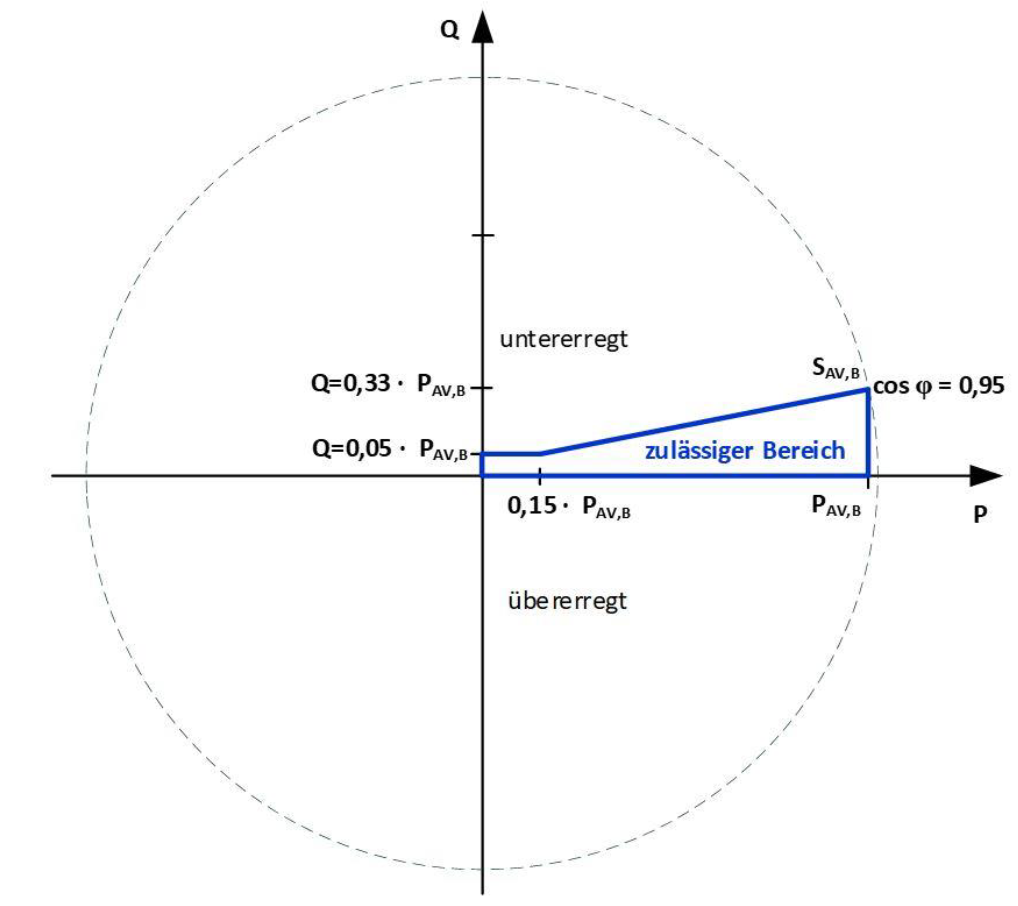
\includegraphics[width=0.6\linewidth]{content/Grafiken/TAR4120_PQ}
	\caption[Zulässiger Bereich des Verschiebungsfaktors cos φ bei Wirkleistungsbezug \cite{VDE4120FNN}]{VDE TAR4120: Zulässiger Bereich des Verschiebungsfaktors}
	\label{fig:tar4120pq}
\end{figure}
Des weiteren sind zeitlich begrenzte Frequenz und Spannungsänderung die auftreten können definiert als quasistationärer Betrieb. Die Netzspannung kann im Bereich von +/- 15 Prozent Schwanken, sowie die Frequenz von 50 Hertz zwischen 47,5 und 51,5 variieren vgl. Abb \ref{fig:vde4120-Anforderungen} (a). Innerhalb dieses Bandes muss die Anlage im regulären Betrieb bleiben. Dabei wird ein Gradient von  <5 \%  im Spannungsband sowie <0,5 \% pro Minute im Frequenzband vorausgesetzt. \\
Im Fehlerfall durch Blitzeinschlag oder Kurzschluss, muss die Anlage kurzzeitig deutlich stärkere Spannungsschwankungen mit machen. Diese Anforderung wird als \gls{FRT} bezeichnet und kann für bis zu 100 Millisekunden die Spannung um 25 Prozent erhöhen vgl. Abb. \ref{fig:vde4120-Anforderungen} (b). Aufgrund eines Kurzschluss kann die Spannung auf 15 Prozent der eigentlichen Netzspannung abfallen. Dies stellt für Verbraucheranlagen eine große Herausforderung dar, da die zu betreibenden Systeme meist eine mindest Spannung benötigen.

\begin{figure}[H]
\centering
\subfloat[][]{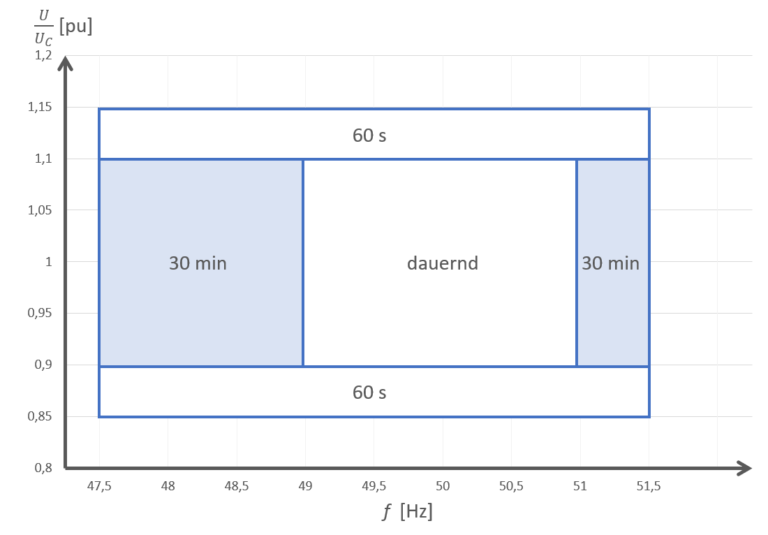
\includegraphics[width=0.7\linewidth]{content/Grafiken/VDE4120-quasistationarerbetrieb}}%
%\caption[Mindestanforderungen an den quasistationären Betrieb von Erzeugungsanlagen \cite{VDEARN4120]{Quasistationärer Betrieb}}

\qquad
\subfloat[][]{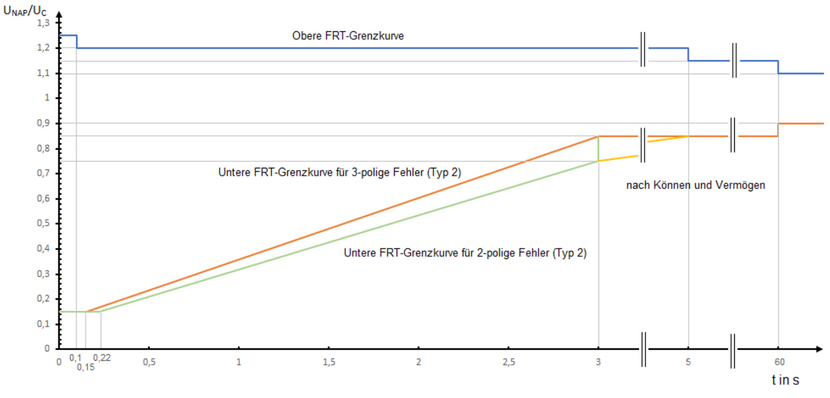
\includegraphics[width=0.7\linewidth]{content/Grafiken/Grenzkurve}}%

\caption[quasistationären Betrieb (a) und \gls{FRT} (b)]{[Mindestanforderungen an den quasistationären Betrieb (a) und \gls{FRT} (b)}
\label{fig:vde4120-Anforderungen}
\end{figure}




\subsection{Systemanforderungen}


\subsection{Überspannungsschutz}

\section{Elektrolyseur}
Zur Elektrolyse wird eine Gleichspannung benötigt welche aufgrund von Alterungsprozessen, innerhalb der Zellmembrane, mit der Zeit ansteigt \cite{HydrogenElectronicTopologies}.
\section{Bewertungskriterien}
Die Kriterien zur finalen Auswahl der Topologie setzen sich aus der Erfüllung der Anforderungen zusammen sowie der Bewertung der Hardware. Die Grundlegenden Anforderungen aus Seiten des Stromnetzes und Elektrolyseur wurden bereits in der Vorauswahl berücksichtigt und können nun im Detail anhand von \gls{THD} und Rippelgrößen betrachtet werden. Die Quantifizierung der Hardware wird zum einen anhand der Verlustleistung in den Halbleitern, welche indirekt auch den Kühlungsaufwand repliziert, zum anderen durch die Größe und den Aufwand für die Komponenten berücksichtigt.  